\begin{center}

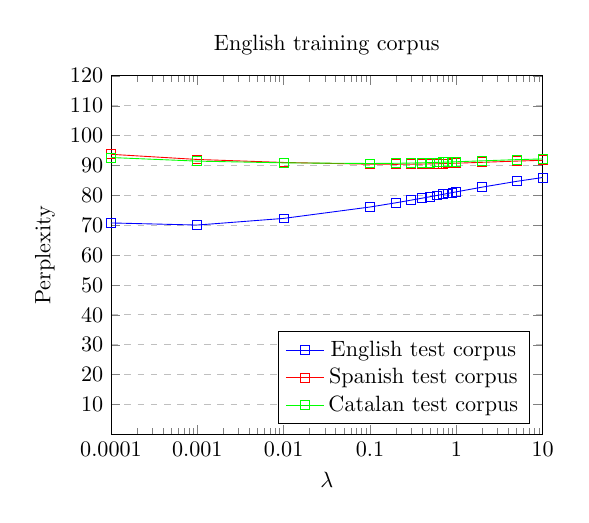
\begin{tikzpicture}[scale=.8]
\begin{semilogxaxis}[
	  log ticks with fixed point,
    title={English training corpus},
    xlabel={$\lambda$},
    ylabel={Perplexity},
    xmin=.0001, xmax=10,
    ymin=0, ymax=120,
    xtick={.0001,.001,.01,.1,1,10},
    ytick={10,20,30,40,50,60,70,80,90,100,110,120},
    legend pos=south east,
    ymajorgrids=true,
    grid style=dashed,
]
 
\addplot[
    color=blue,
    mark=square,
    ]
    coordinates {
(0.00010000,70.7838359216829787)
(0.00100000,70.0739347789917986)
(0.01000000,72.2985689054383442)
(0.10000000,76.1112575719986637)
(0.20000000,77.5275960540965059)
(0.30000000,78.4110212760483734)
(0.40000000,79.0585485541039645)
(0.50000000,79.5700561716805197)
(0.60000000,79.9923144645533739)
(0.70000000,80.3512721271907679)
(0.80000000,80.6629202278716662)
(0.90000000,80.9378480836673617)
(1.00000000,81.1834458751035442)
(2.00000000,82.7700533251326362)
(5.00000000,84.7015648800841063)
(10.00000000,85.9794225151844529)
    };

\addplot[
    color=red,
    mark=square,
    ]
    coordinates {
(0.00010000,93.7409203556402417)
(0.00100000,92.0182444977026819)
(0.01000000,91.0212602048615054)
(0.10000000,90.4230208013376000)
(0.20000000,90.3934129128273582)
(0.30000000,90.4286476652002165)
(0.40000000,90.4789841584193084)
(0.50000000,90.5321812430743336)
(0.60000000,90.5842677606294018)
(0.70000000,90.6338749255175742)
(0.80000000,90.6805991298397771)
(0.90000000,90.7244231639468239)
(1.00000000,90.7654856315493390)
(2.00000000,91.0655139391036812)
(5.00000000,91.4748648613262674)
(10.00000000,91.7415285911387741)
    };

\addplot[
    color=green,
    mark=square,
    ]
    coordinates {
(0.00010000,92.6689697631915124)
(0.00100000,91.4602383881187251)
(0.01000000,90.8863995755205849)
(0.10000000,90.6722033006077055)
(0.20000000,90.7400203907206446)
(0.30000000,90.8239329562637181)
(0.40000000,90.9040457134869371)
(0.50000000,90.9772514576050497)
(0.60000000,91.0435333854303650)
(0.70000000,91.1035665891842683)
(0.80000000,91.1581269891126027)
(0.90000000,91.2079317376320375)
(1.00000000,91.2536028044347347)
(2.00000000,91.5671506411171237)
(5.00000000,91.9590873678890546)
(10.00000000,92.2008818487639275)
    };
    \legend{English test corpus,Spanish test corpus,Catalan test corpus}
 
\end{semilogxaxis}
\end{tikzpicture}
\qquad
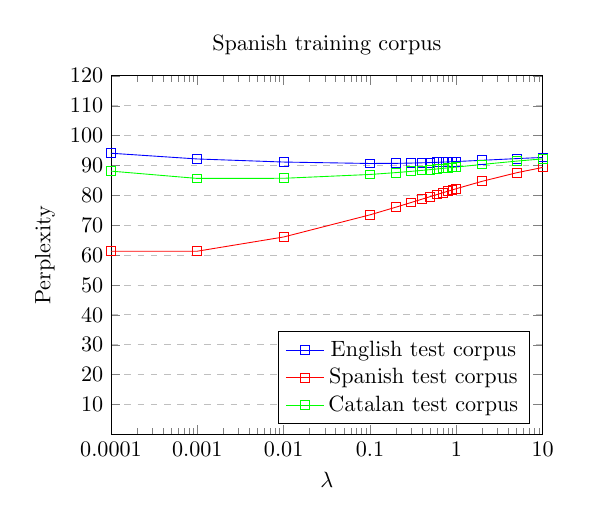
\begin{tikzpicture}[scale=.8]
\begin{semilogxaxis}[
	  log ticks with fixed point,
    title={Spanish training corpus},
    xlabel={$\lambda$},
    ylabel={Perplexity},
    xmin=.0001, xmax=10,
    ymin=0, ymax=120,
    xtick={.0001,.001,.01,.1,1,10},
    ytick={10,20,30,40,50,60,70,80,90,100,110,120},
    legend pos=south east,
    ymajorgrids=true,
    grid style=dashed,
]
 
\addplot[
    color=blue,
    mark=square,
    ]
    coordinates {
(0.00010000,94.1051565833287640)
(0.00100000,92.1852341309041350)
(0.01000000,91.1555916836022817)
(0.10000000,90.6777474967318682)
(0.20000000,90.7210107822816099)
(0.30000000,90.8084710839428340)
(0.40000000,90.8995597802098700)
(0.50000000,90.9860712626818184)
(0.60000000,91.0662574819790933)
(0.70000000,91.1401164525290994)
(0.80000000,91.2081452693207666)
(0.90000000,91.2709504755167131)
(1.00000000,91.3291193874974283)
(2.00000000,91.7438604909954023)
(5.00000000,92.3094410432263146)
(10.00000000,92.6953563315656197)
    };

\addplot[
    color=red,
    mark=square,
    ]
    coordinates {
(0.00010000,61.3100703532033791)
(0.00100000,61.3271455611933831)
(0.01000000,66.0822404749107619)
(0.10000000,73.4898199543197421)
(0.20000000,76.0658873471014658)
(0.30000000,77.6207495700976722)
(0.40000000,78.7352430220479391)
(0.50000000,79.6008155827436212)
(0.60000000,80.3056674646814628)
(0.70000000,80.8980503038770280)
(0.80000000,81.4073356010243145)
(0.90000000,81.8527626210421602)
(1.00000000,82.2476287177819643)
(2.00000000,84.7291104294536410)
(5.00000000,87.5787107352852132)
(10.00000000,89.3461332722549457)
    };

\addplot[
    color=green,
    mark=square,
    ]
    coordinates {
(0.00010000,88.1229201316707673)
(0.00100000,85.6719540751590216)
(0.01000000,85.7197790593851607)
(0.10000000,86.9979904057530149)
(0.20000000,87.6226302067387905)
(0.30000000,88.0435202415742140)
(0.40000000,88.3651218969876595)
(0.50000000,88.6260518476881032)
(0.60000000,88.8455534578886272)
(0.70000000,89.0348029167840025)
(0.80000000,89.2009340469913781)
(0.90000000,89.3488039177523774)
(1.00000000,89.4818791028892804)
(2.00000000,90.3609707510764792)
(5.00000000,91.4675614587979169)
(10.00000000,92.2160959291668405)
    };
    \legend{English test corpus,Spanish test corpus,Catalan test corpus}
 
\end{semilogxaxis}
\end{tikzpicture}

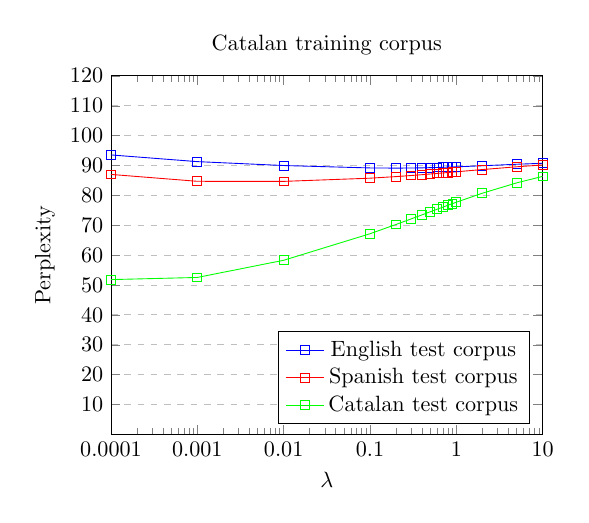
\begin{tikzpicture}[scale=.8]
\begin{semilogxaxis}[
	  log ticks with fixed point,
    title={Catalan training corpus},
    xlabel={$\lambda$},
    ylabel={Perplexity},
    xmin=.0001, xmax=10,
    ymin=0, ymax=120,
    xtick={.0001,.001,.01,.1,1,10},
    ytick={10,20,30,40,50,60,70,80,90,100,110,120},
    legend pos=south east,
    ymajorgrids=true,
    grid style=dashed,
]
 
\addplot[
    color=blue,
    mark=square,
    ]
    coordinates {
(0.00010000,93.5356597887484753)
(0.00100000,91.2953675472633392)
(0.01000000,89.9904532262239485)
(0.10000000,89.1817857495172177)
(0.20000000,89.1281315994347096)
(0.30000000,89.1622677169337408)
(0.40000000,89.2179159825322614)
(0.50000000,89.2786386279231579)
(0.60000000,89.3389844332829881)
(0.70000000,89.3969763822136940)
(0.80000000,89.4519420980331574)
(0.90000000,89.5037442745468184)
(1.00000000,89.5524716136864356)
(2.00000000,89.9129289187149681)
(5.00000000,90.4146778026439506)
(10.00000000,90.7462909859893472)
    };

\addplot[
    color=red,
    mark=square,
    ]
    coordinates {
(0.00010000,87.0130605277985296)
(0.00100000,84.7130529840393081)
(0.01000000,84.6863880013999193)
(0.10000000,85.7540746740866524)
(0.20000000,86.2875977057031776)
(0.30000000,86.6497876759663939)
(0.40000000,86.9274516607664083)
(0.50000000,87.1530142394875611)
(0.60000000,87.3427860385378949)
(0.70000000,87.5063142053992209)
(0.80000000,87.6497309858935694)
(0.90000000,87.7772322391922586)
(1.00000000,87.8918242929521796)
(2.00000000,88.6434976626522655)
(5.00000000,89.5712585312341645)
(10.00000000,90.1864223742098119)
    };

\addplot[
    color=green,
    mark=square,
    ]
    coordinates {
(0.00010000,51.8226074786520314)
(0.00100000,52.5424636600586865)
(0.01000000,58.2870091863047080)
(0.10000000,67.1657819505705618)
(0.20000000,70.2662631977654826)
(0.30000000,72.1383778299454406)
(0.40000000,73.4805756297370607)
(0.50000000,74.5233500242723039)
(0.60000000,75.3728759972319580)
(0.70000000,76.0872099855961608)
(0.80000000,76.7016726637668000)
(0.90000000,77.2393890549036684)
(1.00000000,77.7163359811629562)
(2.00000000,80.7211392303671715)
(5.00000000,84.1925693023529931)
(10.00000000,86.3567220085654270)
    };
    \legend{English test corpus,Spanish test corpus,Catalan test corpus}
 
\end{semilogxaxis}
\end{tikzpicture}

\end{center}